% This is a Basic Assignment Paper but with like Code and stuff allowed in it, there is also url, hyperlinks from contents included. 

\documentclass[11pt]{article}

% Preamble

\usepackage[margin=1in]{geometry}
\usepackage{amsfonts, amsmath, amssymb}
\usepackage{fancyhdr, float, graphicx}
\usepackage[utf8]{inputenc} % Required for inputting international characters
\usepackage[T1]{fontenc} % Output font encoding for international characters
\usepackage{fouriernc} % Use the New Century Schoolbook font
\usepackage[nottoc, notlot, notlof]{tocbibind}
\usepackage{listings}
\usepackage{xcolor}
\usepackage{blindtext}
\usepackage{hyperref}
\hypersetup{
    colorlinks=true,
    linkcolor=black,
    filecolor=magenta,      
    urlcolor=cyan,
    pdfpagemode=FullScreen,
    }

\definecolor{codegreen}{rgb}{0,0.6,0}
\definecolor{codegray}{rgb}{0.5,0.5,0.5}
\definecolor{codepurple}{rgb}{0.58,0,0.82}
\definecolor{backcolour}{rgb}{0.95,0.95,0.92}

\lstdefinestyle{mystyle}{
    backgroundcolor=\color{backcolour},   
    commentstyle=\color{codegreen},
    keywordstyle=\color{magenta},
    numberstyle=\tiny\color{codegray},
    stringstyle=\color{codepurple},
    basicstyle=\ttfamily\footnotesize,
    breakatwhitespace=false,         
    breaklines=true,                 
    captionpos=b,                    
    keepspaces=true,                 
    numbers=left,                    
    numbersep=5pt,                  
    showspaces=false,                
    showstringspaces=false,
    showtabs=false,                  
    tabsize=2
}

\lstset{style=mystyle}

% Header and Footer
\pagestyle{fancy}
\fancyhead{}
\fancyfoot{}
\fancyhead[L]{\textit{\Large{Information and Cycbersecurity - 2nd Year B. Tech}}}
%\fancyhead[R]{\textit{something}}
\fancyfoot[C]{\thepage}
\renewcommand{\footrulewidth}{1pt}



% Other Doc Editing
% \parindent 0ex
%\renewcommand{\baselinestretch}{1.5}

\begin{document}

\begin{titlepage}
    \centering

    %---------------------------NAMES-------------------------------

    \huge\textsc{
        MIT World Peace University
    }\\

    \vspace{0.75\baselineskip} % space after Uni Name

    \LARGE{
        Information and Cybersecurity\\
        Second Year B. Tech, Semester 1
    }

    \vfill % space after Sub Name

    %--------------------------TITLE-------------------------------

    \rule{\textwidth}{1.6pt}\vspace*{-\baselineskip}\vspace*{2pt}
    \rule{\textwidth}{0.6pt}
    \vspace{0.75\baselineskip} % Whitespace above the title



    \huge{\textsc{
            Message Integrity Checks\\
            \textit{(Message Digest Method - 5) MD5 and \\ (Secure Hashing Algorithm) SHA-256}
        }} \\



    \vspace{0.5\baselineskip} % Whitespace below the title
    \rule{\textwidth}{0.6pt}\vspace*{-\baselineskip}\vspace*{2.8pt}
    \rule{\textwidth}{1.6pt}

    \vspace{1\baselineskip} % Whitespace after the title block

    %--------------------------SUBTITLE --------------------------	

    \LARGE\textsc{
        Lab Assignment 5
    } % Subtitle or further description
    \vfill

    %--------------------------AUTHOR-------------------------------

    Prepared By
    \vspace{0.5\baselineskip} % Whitespace before the editors

    \Large{
        Krishnaraj Thadesar \\
        Cyber Security and Forensics\\
        Batch A1, PA 20
    }


    \vspace{0.5\baselineskip} % Whitespace below the editor list
    \today

\end{titlepage}


\tableofcontents
\thispagestyle{empty}
\clearpage

\setcounter{page}{1}

\section{Aim}
Write a program using JAVA or Python or C++ to implement integrity of message using
MD5 or SHA

\section{Objectives}
To use of hashing algorithm to check message integrity.

\section{Theory}

\subsection{Secure Hashing Algorithm (SHA-256)}

\begin{figure}[H]
    \centering
    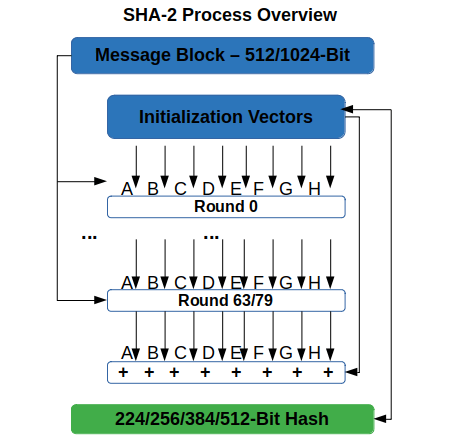
\includegraphics[width=0.55\textwidth]{how-the-sha2-hashing-algorithm-works.png}
    \caption{Working of SHA-256}
\end{figure}

\textit{SHA-256 is a widely used cryptographic hash function that generates a 256-bit (32-byte) digest or hash value from an input message.}

Here are the steps involved in the SHA-256 algorithm:

\begin{enumerate}
    \item \textbf{Message padding}: The input message is padded so that its length is a multiple of 512 bits, which is the block size used by SHA-256. The padding scheme used by SHA-256 is similar to the one used by SHA-1, but with some modifications.

    \item \textbf{Initialize hash values}: SHA-256 uses eight initial hash values, represented as 32-bit words. These values are specified in the SHA-256 specification and are typically denoted as H0, H1, H2, H3, H4, H5, H6, and H7.

    \item \textbf{Process message in 512-bit blocks}: The padded message is divided into 512-bit blocks, and each block is processed by the SHA-256 algorithm.

    \item \textbf{Initialize working variables}: SHA-256 uses a set of working variables, represented as 32-bit words, to store intermediate values during the hashing process. These working variables are typically denoted as a, b, c, d, e, f, g, and h.

    \item \textbf{Compute the hash}: For each 512-bit block, SHA-256 performs 64 rounds of computation to update the working variables and generate the hash value. Each round involves several operations, including bitwise operations, logical operations, and modular addition. The specific operations used in SHA-256 are designed to provide strong cryptographic properties, such as collision resistance and preimage resistance.

    \item \textbf{Combine hash values}: After processing all blocks in the message, the final hash value is computed by combining the eight 32-bit hash values computed during the process. This is typically done by concatenating the hash values in the order H0, H1, H2, H3, H4, H5, H6, and H7 to obtain the 256-bit SHA-256 digest.
\end{enumerate}

\subsection{Example}

\begin{enumerate}
    \item here is an example of how SHA-256 can be used to generate a hash value from a sample input message "Hello, world!":

    \item \textbf{Message Padding}: The ASCII encoding of the message is "48656c6c6f2c20776f726c6421". To pad the message to a length that is a multiple of 512 bits, the message is first appended with a single "1" bit, followed by as many "0" bits as necessary to make the length of the message 448 bits (56 bytes less than a multiple of 512). Then, the original length of the message in bits (80 bits in this case) is added as a 64-bit big-endian integer. Therefore, the padded message is:

          48656c6c6f2c20776f726c64210000000000000000000000000000000000000000000\\
          00000000000000000000005000

    \item \textbf{Initialize Hash Values}: The initial hash values for SHA-256 are specified in the SHA-256 specification and are typically denoted as H0, H1, H2, H3, H4, H5, H6, and H7:

          H0 = 6a09e667
          H1 = bb67ae85
          H2 = 3c6ef372
          H3 = a54ff53a
          H4 = 510e527f
          H5 = 9b05688c
          H6 = 1f83d9ab
          H7 = 5be0cd19

    \item \textbf{Process Message in 512-bit Blocks}: The padded message is divided into 512-bit blocks, and each block is processed by the SHA-256 algorithm. In this case, there is only one block since the message is short enough to fit into a single block.

    \item \textbf{Initialize Working Variables}: SHA-256 uses a set of working variables, represented as 32-bit words, to store intermediate values during the hashing process. These working variables are typically denoted as a, b, c, d, e, f, g, and h:

          a = H0
          b = H1
          c = H2
          d = H3
          e = H4
          f = H5
          g = H6
          h = H7

    \item \textbf{Compute the Hash}: For each 512-bit block, SHA-256 performs 64 rounds of computation to update the working variables and generate the hash value. Each round involves several operations, including bitwise operations, logical operations, and modular addition. Here is a summary of the operations for the first block:

    \item \textbf{Divide the block into 16 32-bit words, denoted as W[0] through W[15]}:
          Compute W[i] for i from 16 to 63 using the formula: sigma1(W[i-2]) + W[i-7] + sigma0(W[i-15]) + W[i-16], where sigma0 and sigma1 are specific bitwise operations used in SHA-256.
          Initialize temporary variables T1 and T2 to a and e, respectively.
          Perform 64 rounds of computation using the formulae:
          T1 = h + Sigma1(e) + Ch(e, f, g) + K[i] + W[i]
          T2 = Sigma0(a) + Maj(a, b, c)

    \item \textbf{Finalize Hash Value}: After processing all of the blocks, the final hash value is computed by concatenating the values of a, b, c, d, e, f, g, and h, in that order, and converting each 32-bit word to a 4-byte big-endian integer. In this example, the final hash value is:

          0x7cf5d5e440b5d760b5a22d9b759f4419f544e1e7525ccae037ba20a8d1e26c35
\end{enumerate}


\section{Platform}
\textbf{\textbf{Operating System}}: Arch Linux x86-64 \\
\textbf{\textbf{IDEs or Text Editors Used}}: Visual Studio Code\\
\textbf{\textbf{Compilers or Interpreters} }: Python 3.10.1\\

\section{Input and Output}
\begin{verbatim}
Hash of the file is: 
b91bf2a1dd825725f788a7e204cfd38d0a4badd1bf3745ec2efceeb4e3cab591
Modified the File, added hidden data to it.
Hash of the file now is: 
d02d021cc9c7771339327216c82540b1796ce1f2d715797907c97ee7c24788e8
\end{verbatim}
\section{Code}
\lstinputlisting[language=Python, caption="SHA Integrity Check"]{../Programs/Assignment_5/sha.py}

\section{Conclusion}
Thus, learnt about the different types of message integrity checks and how to implement them in Python.
MD5 and SHA are the most commonly used message integrity checks, and were implemented in this assignment using the hashlib library.

\clearpage

\section{FAQ}

\begin{enumerate}
    \item \textit{What is MAC? What is the difference between MAC and message digest.} \\

          \textbf{\textbf{Definition}}: \\

          \textbf{MAC} stands for \textit{Message Authentication Code}, and it is \textit{a type of cryptographic technique used to provide integrity and authenticity of a message.} A MAC is generated by taking a secret key and combining it with the message using a cryptographic hash function or a symmetric encryption algorithm. The resulting MAC is appended to the message and sent along with it. The receiver can then use the same secret key and cryptographic algorithm to compute the MAC and verify that it matches the MAC sent with the message, thus ensuring the integrity and authenticity of the message.

          A \textbf{message digest}, on the other hand, is \textit{a fixed-length output generated by applying a cryptographic hash function to a message.} The resulting digest can be used to verify that the message has not been tampered with, but it does not provide authentication. A message digest can be thought of as a digital fingerprint of a message, which is unique to that message and can be used to identify any changes made to the message.\\


          \textbf{Differences}:\\

          \begin{enumerate}
              \item \textbf{Purpose}: The purpose of MAC is to provide both integrity and authenticity of a message, while the purpose of a message digest is to provide integrity only.

              \item \textbf{Technique}: MAC uses a secret key and a cryptographic algorithm such as a hash function or a symmetric encryption algorithm to create a unique code that authenticates the message. In contrast, message digest only uses a cryptographic hash function to generate a fixed-length output that verifies the integrity of the message.

              \item \textbf{Key Requirements}: MAC requires a secret key that is shared between the sender and receiver to generate the code, while message digest only requires a publicly available cryptographic hash function.

              \item \textbf{Strength}: MAC provides stronger authentication than message digest because it uses a secret key to create a unique code that cannot be forged. Message digest, on the other hand, only provides integrity verification and can be more susceptible to attacks.

              \item \textbf{Resource Requirements}: MAC requires more computational resources than message digest because it uses a cryptographic algorithm that requires more processing power. Additionally, MAC requires a secure key distribution channel, which can add to the resource requirements.

              \item \textbf{Usage}: MAC is commonly used in secure communication protocols such as SSL/TLS, IPSec, and SSH, while message digest is commonly used for verifying file integrity, password storage, and digital signatures.
          \end{enumerate}


    \item \textit{Compare MD5 and SHA-1.} \\
          MD5 and SHA1 are both cryptographic hash functions that are used to generate a fixed-length output, or digest, from a message. Here are some differences between MD5 and SHA1:

          \begin{enumerate}
              \item \textbf{Output size}: MD5 generates a 128-bit digest, while SHA1 generates a 160-bit digest. This means that SHA1 is slightly stronger than MD5 in terms of the number of possible output values.

              \item \textbf{Collision resistance}: MD5 is considered to be weak in terms of collision resistance, which means that it is possible to generate two different messages that produce the same MD5 digest. SHA1 is also vulnerable to collision attacks, but it is considered to be stronger than MD5.

              \item \textbf{Speed}: MD5 is generally faster than SHA1 because it uses a simpler algorithm. However, because of its weaknesses, it is no longer recommended for use in security-sensitive applications. SHA1 is slightly slower than MD5 but is still considered to be a fast and efficient hash function.

              \item \textbf{Usage}: MD5 was once widely used in security applications such as digital signatures and password storage, but it is now considered to be insecure and should be avoided. SHA1 is still commonly used for data integrity and message authentication, but it is gradually being phased out in favor of stronger hash functions such as SHA-256 and SHA-3.

              \item \textbf{Security}: Both MD5 and SHA1 are considered to be weak and vulnerable to attacks by modern computing resources, which can compromise their security in practical applications. As a result, it is recommended to use stronger cryptographic hash functions, such as SHA-256 or SHA-3, for security-sensitive applications.
          \end{enumerate}

    \item \textit{Compare various versions of SHA.} \\

          There are several versions of the SHA (Secure Hash Algorithm) family of cryptographic hash functions, each with different strengths and output sizes. Here is a comparison of some of the most widely used SHA versions:

          \begin{enumerate}
              \item \textbf{SHA-1}: SHA-1 is a 160-bit hash function that was widely used for data integrity and message authentication. However, it is now considered to be vulnerable to collision attacks and has been deprecated in favor of stronger hash functions.

              \item \textbf{SHA-2}: SHA-2 is a family of hash functions that includes SHA-224, SHA-256, SHA-384, and SHA-512, each with different output sizes. SHA-256 is a 256-bit hash function that is widely used for digital signatures, file verification, and other security applications. SHA-384 and SHA-512 are designed for use in applications that require a higher level of security, such as secure communications and financial transactions.

              \item \textbf{SHA-3}: SHA-3 is the latest addition to the SHA family of hash functions, and was developed as a result of the NIST hash function competition. It is a family of hash functions that includes SHA3-224, SHA3-256, SHA3-384, and SHA3-512, each with different output sizes. SHA-3 is designed to be more secure and efficient than previous versions of SHA.

          \end{enumerate}

          \begin{enumerate}
              \item \textbf{Output size}: SHA-1 generates a 160-bit digest, SHA-2 generates a range of digest sizes from 224 to 512 bits, while SHA-3 also generates a range of digest sizes from 224 to 512 bits. Generally, larger output sizes provide stronger security and are more resistant to collision attacks.

              \item \textbf{Collision resistance}: SHA-1 has been found to be vulnerable to collision attacks, while SHA-2 and SHA-3 are designed to be more resistant to such attacks. SHA-3 is particularly strong in this regard due to its sponge construction.

              \item \textbf{Algorithm}: SHA-1, SHA-2, and SHA-3 all use different algorithms to generate their digests. SHA-1 and SHA-2 use a Merkle-Damgård construction, while SHA-3 uses a sponge construction. The sponge construction provides better resistance against attacks, such as length extension attacks, that can affect Merkle-Damgård construction.

              \item \textbf{Performance}: SHA-2 and SHA-3 generally require more processing power than SHA-1 due to their larger digest sizes and more complex algorithms. However, the performance difference may be insignificant in practice, and the security benefits of using SHA-2 or SHA-3 may outweigh the performance costs.

              \item \textbf{Standardization}: SHA-1 and SHA-2 are widely standardized and have been widely used in various security applications, while SHA-3 is a relatively new standard and has yet to gain widespread adoption.

              \item \textbf{Security}: SHA-1 is now considered insecure and should not be used in security-sensitive applications. SHA-2 and SHA-3 are considered to be secure and are recommended for use in security-sensitive applications, with SHA-3 being the stronger choice.
          \end{enumerate}


\end{enumerate}

\end{document}